\newpage
\chapter{Integración de sistema}

\section{Introducción}

La integración del sistema representa el punto culminante del desarrollo del proyecto, reuniendo todos los componentes implementados a lo largo de las iteraciones previas en una solución cohesiva y funcional, además busca garantizar que cada componente contribuya de forma efectiva al cumplimiento de los objetivos del proyecto. Hasta el momento, se ha logrado consolidar un prototipo de robot omnidireccional con un sistema de control compensado, un mapa estructurado gobernado por un conjunto red de Petri/Monitor, una interfaz de usuario que permite el monitoreo y supervisión de las operaciones del robot, además de introducir el Filtro de Kalman para mejorar la precisión en la estimación de la posición del mismo.

En esta etapa, el objetivo central es integrar estos elementos en un sistema completo que opere de manera armónica y eficiente, optimizando su desempeño y consolidando su capacidad para interactuar en el entorno modelado.

\section{Resultados de iteraciones previas}

Durante el desarrollo se realizaron un número de iteraciones que condujeron al resultado final de la integración. A continuación se presenta un resumen de los hallazgos obtenidos en las iteraciones incrementales y cómo estas contribuyeron a la integración final.

\begin{itemize}
    \item Iteración 0: Decisiones preliminares
    \begin{itemize}
        \item Elección del microcontrolador
        \item Elección de motores y sensores rotativos
        \item Elección del lenguaje para interfaz
        \item Elección del protocolo para comunicaciones
    \end{itemize}

    \item Iteración 1: Prototipo del robot
    \begin{itemize}
        \item Sistema de control PID en cada rueda
        \item Movimientos con el Modelo Cinemático
        \item Cálculo de odometría
        \item Envío y recepción de comandos inalámbricos
    \end{itemize}

    \item Iteración 2: Prototipo mejorado
    \begin{itemize}
        \item Modelo Cinemático compensado
        \item Seguidor de línea
    \end{itemize}

    \item Iteración 3: Modelo del mapa e interfaz
    \begin{itemize}
        \item Interfaz de usuario
        \item Modelo del mapa y diseño de la pista
        \item Calculador de trayectorias
    \end{itemize}

    \item Iteración 4: Red de Petri y Monitor
    \begin{itemize}
        \item Modelo del mapa con una Red de Petri
        \item Monitor concurrente
    \end{itemize}

    \item Iteración 5: Filtro de Kalman
    \begin{itemize}
        \item Implementación del Filtro de Kalman
        \item Compensación con estimación de Kalman
    \end{itemize}

    \item Iteración 6: Mediciones con códigos QR
\end{itemize}


\section{Componentes del sistema}

Una vez integrados todos los componentes, podemos plasmar cómo se relacionan entre sí en la Figura \ref{fig:integsistemadiagcomp} mediante un diagrama de bloques.

\begin{figure}[H]
    \centering
    \hspace*{-2.0cm}
    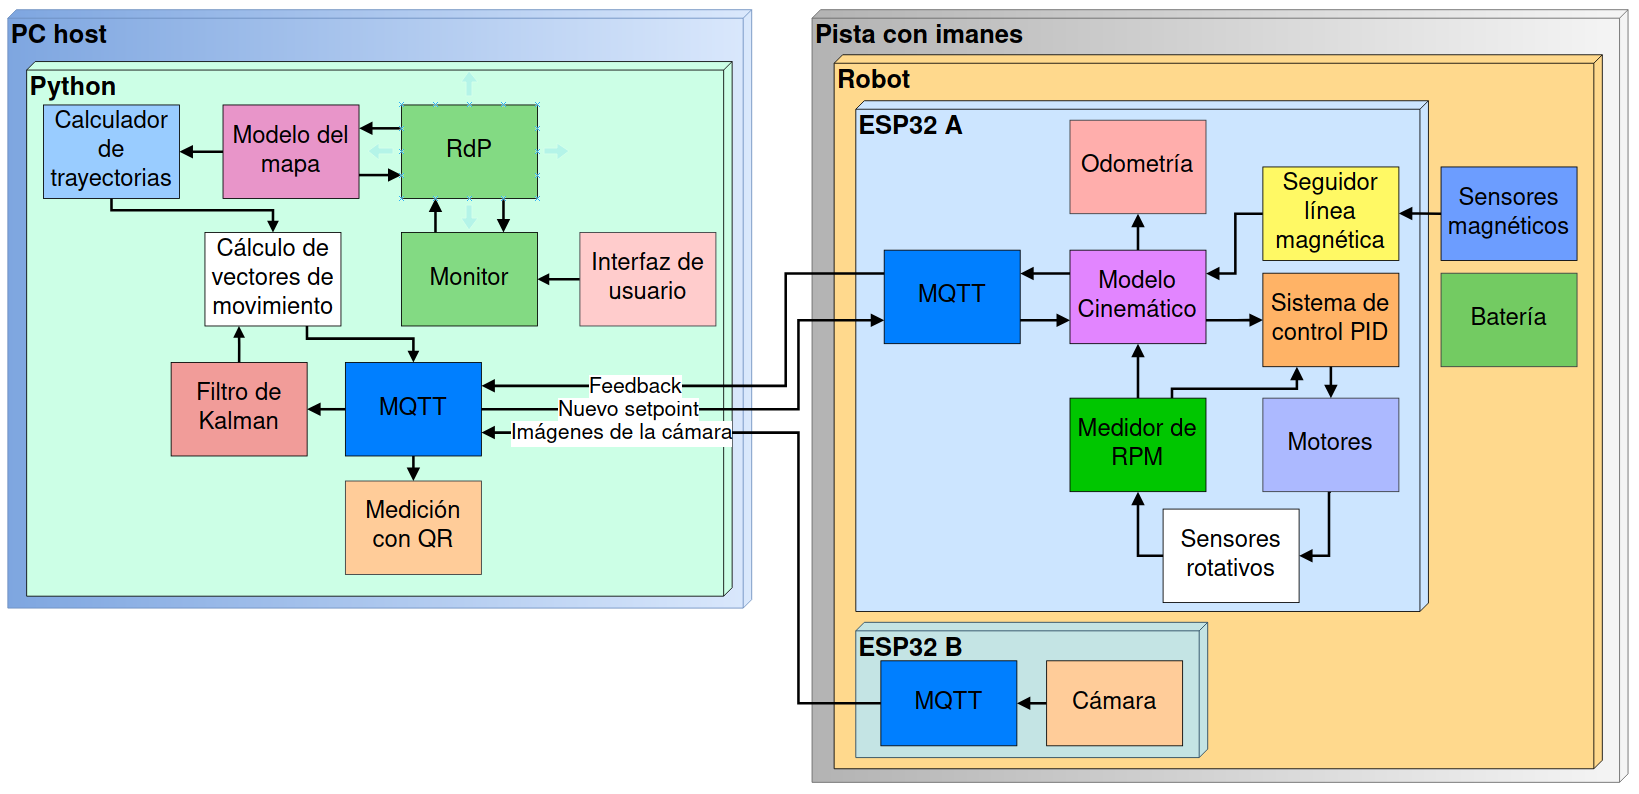
\includegraphics[width=1.25\linewidth]{images/integ_sistema_general.png}
    \caption{Diagrama de componentes del sistema}
    \label{fig:integsistemadiagcomp}
\end{figure}


\subsection{Compensaciones y lazos de realimentación}

Hasta el momento resulta claro que nuestro proyecto integra múltiples mecanismos para lograr que el movimiento del robot sea lo más efectivo posible. En diferentes niveles, cada sistema de compensación actúa sobre la señal que recibe cada rueda al realizar movimientos. De menor a mayor en nivel de jerarquía, tenemos:

\begin{itemize}
    \item Sistema de control PID por cada rueda.
    \item Modelo cinemático compensado.
    \item Seguidor de línea magnético.
    \item Filtro de Kalman compensado.
\end{itemize}

En resumen, podemos describir todos los mecanismos de compensación del robot mediante el diagrama de la Figura \ref{fig:integsistemalazosrealim}.

\begin{figure}[H]
    \centering
    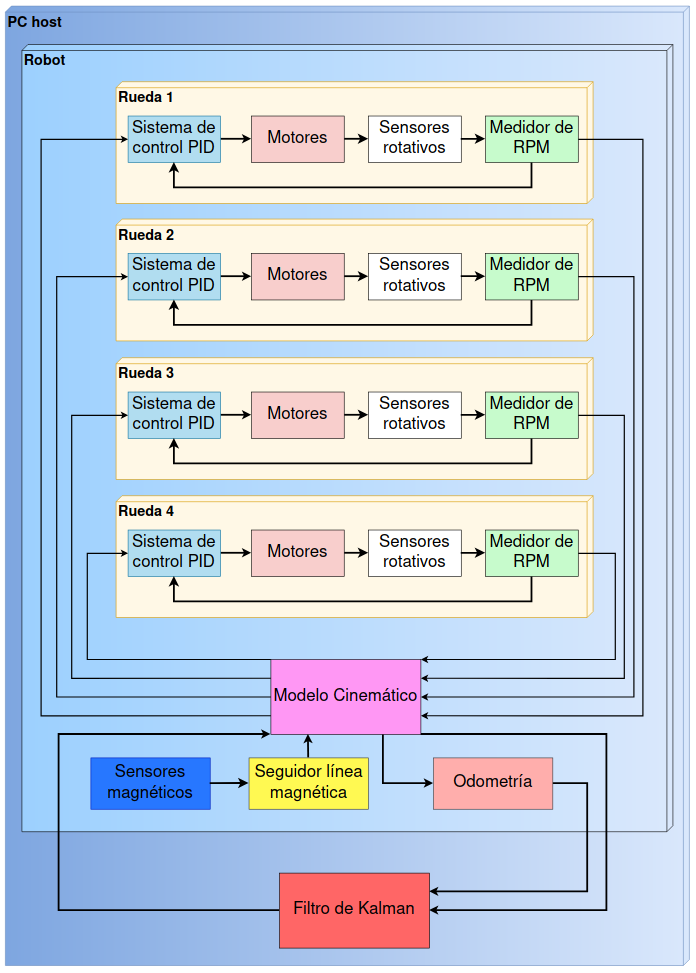
\includegraphics[width=0.8\linewidth]{images/integ_sistema_diag_compensacion.png}
    \caption{Lazos de realimentación intervinientes}
    \label{fig:integsistemalazosrealim}
\end{figure}


\subsection{Entorno del robot y composición final}

Por más que nuestro proyecto está en gran medida orientado hacia la realización de un prototipo de robot, tenemos que el sistema completo es un conjunto de varios elementos distribuidos, como ser el robot en sí, la pista con imanes, los códigos QR y la PC host.

Es por ello que procedemos a ilustrar cómo el robot interactúa con el resto de los elementos para lograr la funcionalidad completa. En primer lugar, tenemos el robot colocado en la pista con imanes. El vano central corresponde al obstáculo representado en la interfaz del mapa y es un lugar no transitable. Al mismo tiempo, se colocan los códigos QR a una altura adecuada en puntos estratégicos para que el robot los lea en puntos clave del mapa.

\begin{figure}[H]
    \centering
    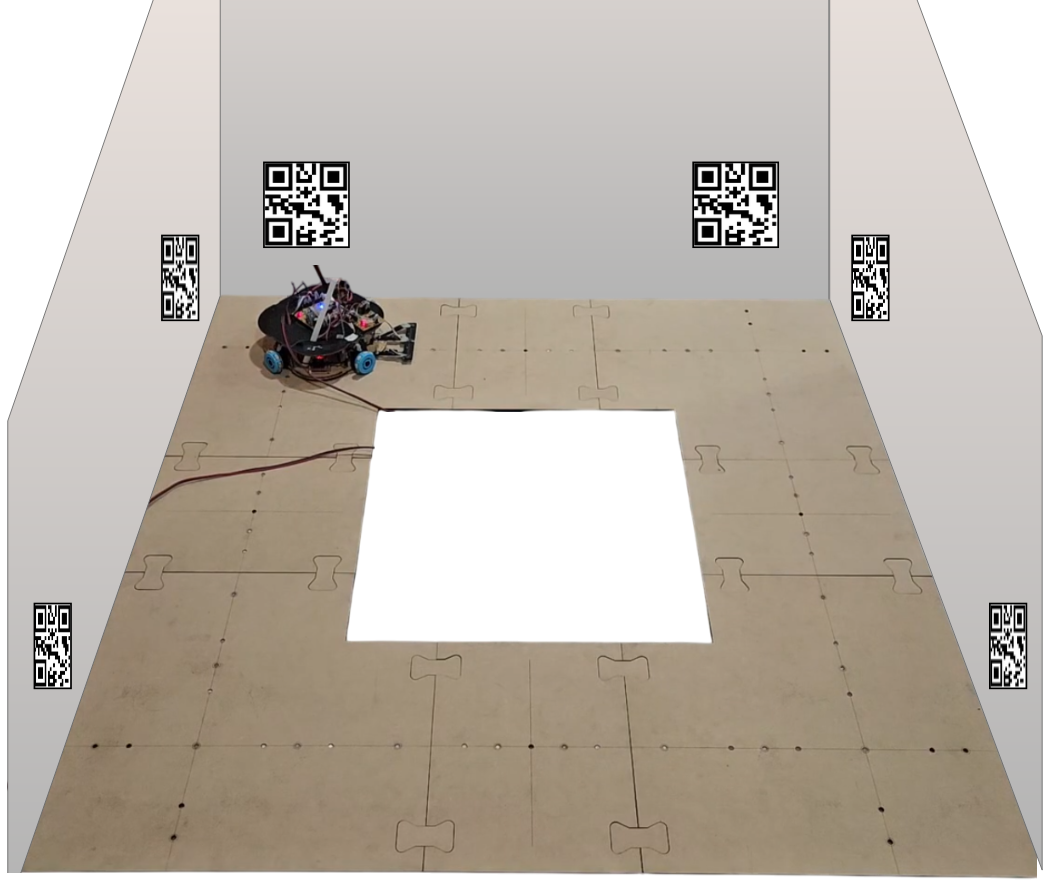
\includegraphics[width=0.75\linewidth]{images/integ_sistema_robot_en_plano.png}
    \caption{Robot en la pista con imanes y entorno con códigos QR}
    \label{fig:integsistemarobotpistaqr}
\end{figure}

En la Figura \ref{fig:integsistemainterfaz} podemos ver en la PC host la representación en tiempo real del robot en el mapa. Su orientación se denota con una flecha en esa dirección y también el nombre del robot que ocupa la celda.

Finalmente, en la Figura \ref{fig:integsistemainterfazgrafana} se describe la interfaz que nos permite monitorear velocidades y posición del robot y visualizar las imágenes capturadas por la cámara.

En el cuadro superior izquierdo tenemos la captura de imágenes de la cámara. En el cuadro superior derecho tenemos una representación de las velocidades lineales y rotacionales, además de las distancias recorridas, en función del tiempo.

En el cuadro inferior izquierdo se observa la salida del lector de códigos QR, donde periódicamente utiliza la última imagen capturada y detecta si existe un código QR en ella o no y cuál es su \textit{payload}. Finalmente, en el cuadro inferior derecho se observa la representación de la trayectoria recorrida hasta el momento, basada en las estimaciones del Filtro de Kalman.

\begin{figure}[H]
    \centering
    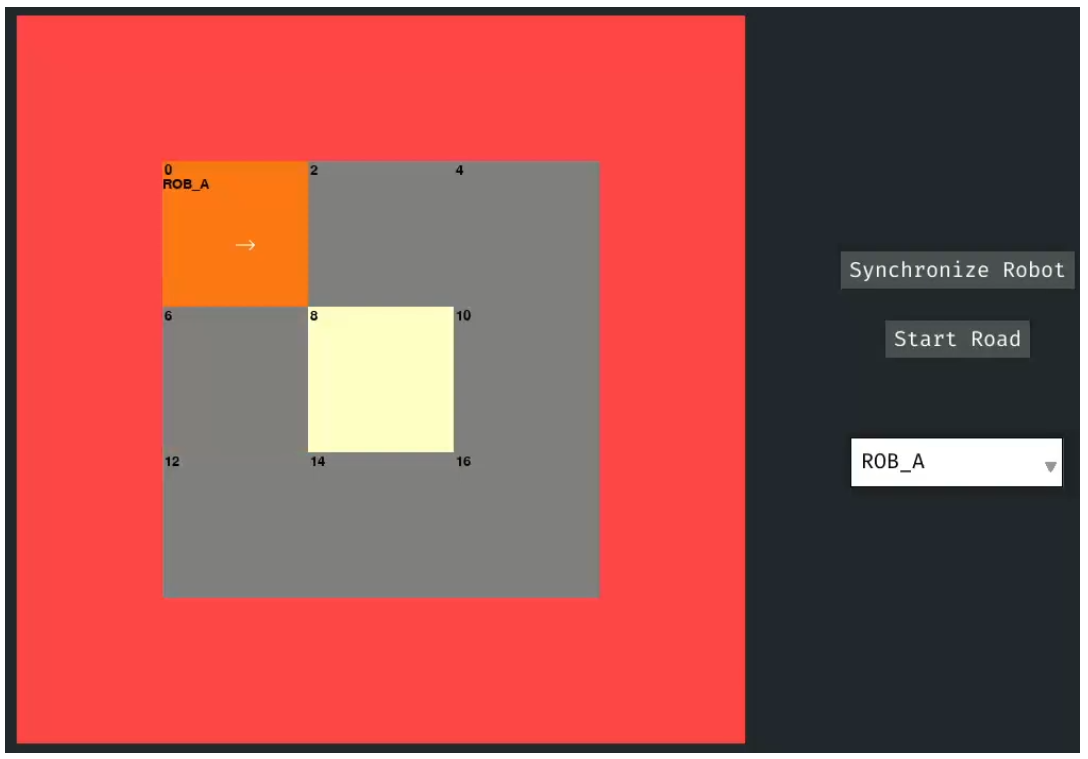
\includegraphics[width=0.8\linewidth]{images/integ_sistema_interfaz_python.png}
    \caption{Monitoreo del robot en tiempo real}
    \label{fig:integsistemainterfaz}
\end{figure}

\begin{figure}[H]
    \centering
    \hspace*{-1.1cm}
    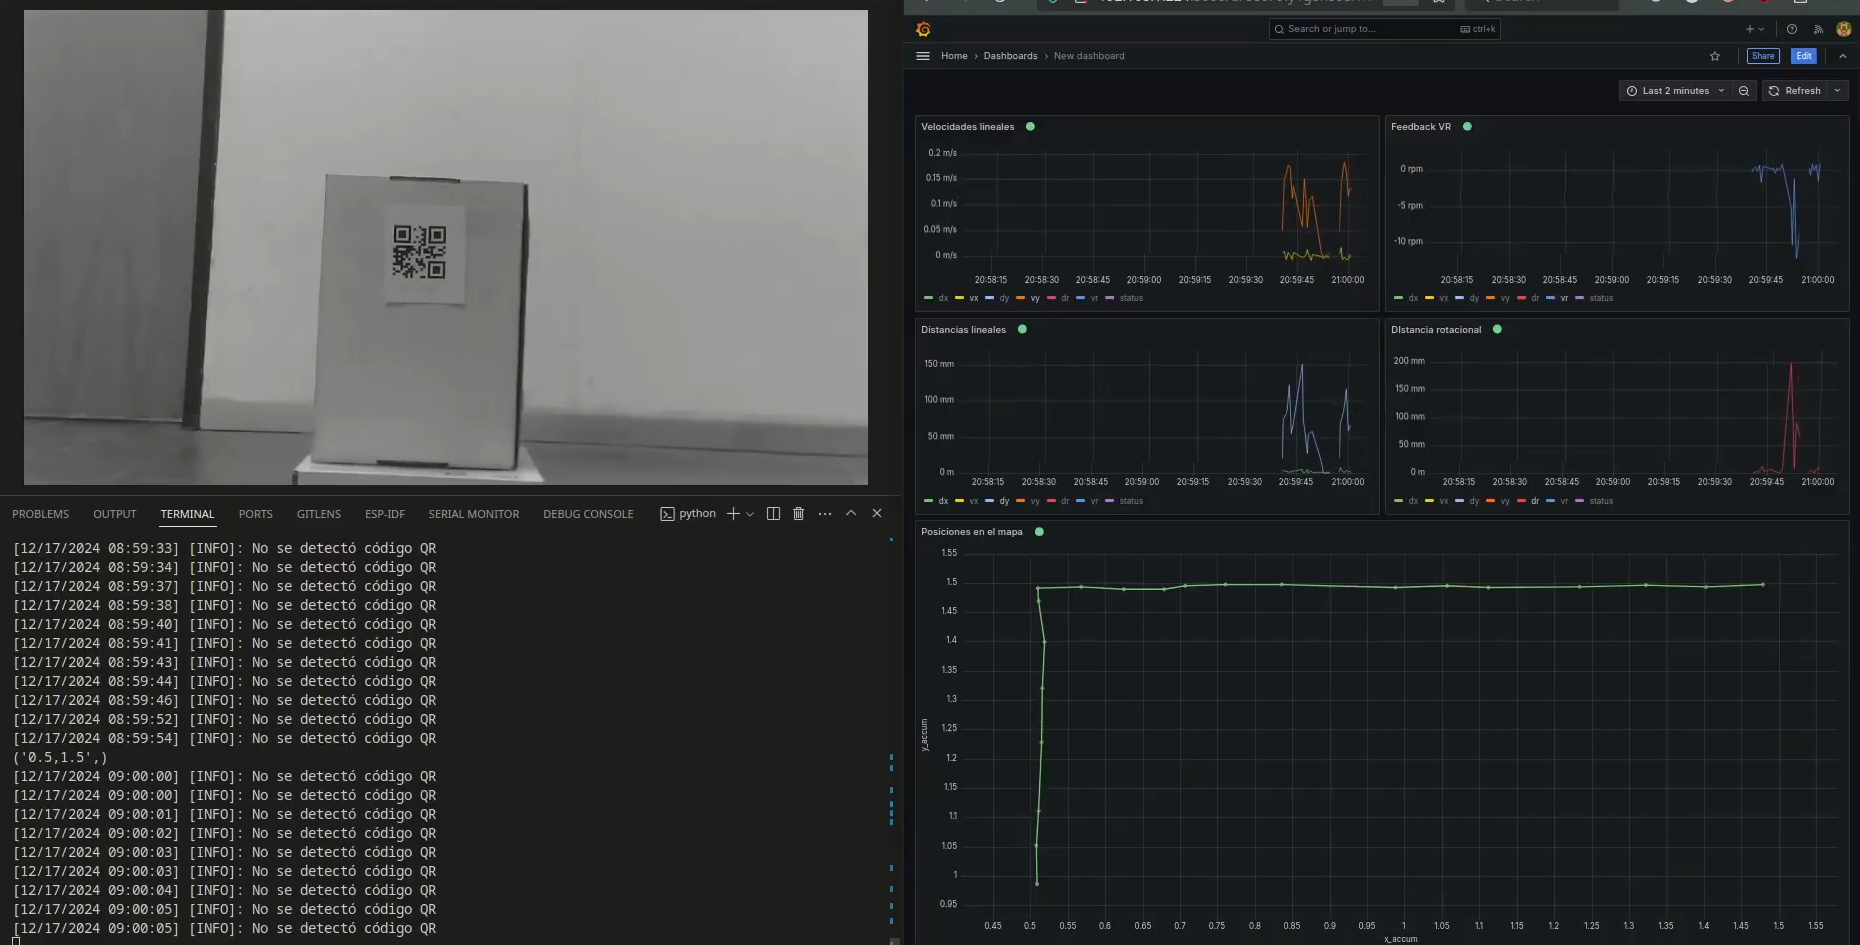
\includegraphics[width=1.2\linewidth]{images/integ_sistema_interfaz_camara_grafana.png}
    \caption{Monitoreo de estimación de Kalman, obtención y procesamiento de códigos QR}
    \label{fig:integsistemainterfazgrafana}
\end{figure}


\section{Problemas enfrentados}

Una vez realizadas todas las iteraciones del desarrollo, al momento de realizar la integración final del sistema se encontraron algunas situaciones donde el robot no se comportaba adecuadamente debido a desperfectos en el software, hardware o ajustes mecánicos; procedimos a realizar las correcciones y se concretó la integración. Se mencionan algunos de los mayores problemas enfrentados:

\begin{itemize}
    \item \underline{Medición de RPM a bajas velocidades:} al implementar el medidor de RPM vimos que las mediciones a bajas RPM eran inexactas, por lo que debimos implementar una solución acumulativa que no es altamente precisa, pero lo suficiente para nuestra aplicación. Esto se debe a limitaciones para fabricar un encoder de precisión.

    \item \underline{Mecanismo para seguidor de línea magnético:} para la realización del seguidor de línea magnético debimos iterar un número de veces dado que las técnicas propuestas no resultaban efectivas, hasta que finalmente convergimos en la solución de una compensación rotacional adaptativa.

    \item \underline{Dependencia de comunicación inalámbrica para compensación del Filtro de Kalman:} dado que el robot reporta feedback por medio de MQTT y el Filtro de Kalman envía compensaciones por el mismo medio, existen casos donde hay algunos retardos en el envío de datos y ocasiona correcciones tardías, generando desviaciones en la trayectoria.

    \item \underline{Limitaciones de Python para granularidad fina de hilos:} en Python todos los hilos que se crean son de cierto modo "virtuales". Esto es porque existe un semáforo global llamado GIL que en round-robin le da recursos a cada hilo periódicamente. En nuestro caso esto es un limitante porque tuvimos que recurrir a elaborar mecanismos para poder despertar o poner en espera un hilo determinado.    
\end{itemize}


\section{Testing y verificación}

Las pruebas de integración y de sistema fueron realizadas a lo largo de cada una de las iteraciones y se reflejan en los casos de prueba:

\begin{itemize}
    \item TC\_01\_09
    \item TC\_02\_03
    \item TC\_05\_06
    \item \textbf{FIXME faltan los de la iteracion 4 y 6}
\end{itemize}


\section{Puntos de mejora}

Durante el desarrollo del proyecto se encontraron varios aspectos en los que se puede mejorar el robot, ya sea en el movimiento, comunicación o hardware. A continuación se listan algunos de los puntos que han sido detectados:

\begin{itemize}
    \item Utilizar motores con hoja de datos: de este modo se lograría tener un sistema de control PID exacto para el motor y se obtendría una mejor integración y movimiento.

    \item Utilizar técnicas avanzadas para detectar deslizamiento de las ruedas: en la bibliografía \cite{phunopasomnirobot} \cite{palacinodometry} se detallan algunos métodos para poder detectar y corregir estas situaciones. No han sido implementadas en este proyecto por escapar al alcance del mismo.
    
    \item Integrar mejores encoders rotativos para medición de RPM: esto se puede lograr ya sea mejorando el diseño propuesto para los sensores o utilizando sensores comerciales.
    
    \item Mejoras en el chasis: la carrocería del robot puede ser mejorada de modo que contenga mejor los componentes internos y puede incluir de modo nativo el soporte para la cámara.
    
    \item Buscar un modo para usar un solo microcontrolador ESP32 en lugar de utilizar uno para el control cinemático y otro para la cámara.
\end{itemize}
